\documentclass{article}

\bibliographystyle{plain}
\usepackage[final]{nips_2017}
\usepackage[utf8]{inputenc} % allow utf-8 input
\usepackage[T1]{fontenc}    % use 8-bit T1 fonts
\usepackage{hyperref}       % hyperlinks
\usepackage{url}            % simple URL typesetting
\usepackage{booktabs}       % professional-quality tables
\usepackage{amsfonts}       % blackboard math symbols
\usepackage{nicefrac}       % compact symbols for 1/2, etc.
\usepackage{microtype}      % microtypography
\usepackage{graphicx}
\usepackage{amsmath}
\usepackage{enumitem}
\usepackage{caption}
\usepackage{subcaption}
\usepackage{float}
\usepackage{comment}
\usepackage{multicol}
\allowdisplaybreaks
\raggedbottom

\title{Modelling State-of-Health for a Li-ion Battery}
\author{Karthik Nataraj, Hampus Carlens and Julian Cooper}

\begin{document}

\maketitle

\section{Motivation}
Lithium ion batteries are of great and increasing importance in today's society due to their high energy density.  Li-on batteries' performance capability can be characterized by their State of Health (SOH). SOH is a measure of usable capacity over rated capacity. Accurately predicting how many cycles (i.e charge then discharge) a battery can perform, at any given time, before reaching it’s end of useful life is important for reliability. However, prediction is notoriously difficult due to poor understanding of how the measurable parameters (voltage, current, temperature, etc.) effect the SOH. Today three main methods are used: electrochemical, equivalent circuit, and data-driven models.

There have been many previous studies into data-driven models for SOH prediction. Some of the most cited recent publications are \cite{severson2019data}, \cite{roman2021machine} and \cite{energiesMdpi}, all of which produce predictors for RUL with Mean Absolute Percentage Error (MAPE) ranging from 2-15\%.  The lowest errors are obtained using deep neural networks such as in \cite{roman2021machine} and \cite{energiesMdpi}, with MAPE of $~ 2\%$. Multiple authors (including \cite{energiesMdpi} and \cite{DariusOld}) point towards the importance of future work in trying to scale these models, to make them suitable for front-end embedded systems. In \cite{severson2019data} the authors opt for a simple linear model over neural networks. Given information from the first 100 cycles only, they manage to achieve MAPE of 13\% for RUL predictions. 

In this project, we develop a scalable (and explainable) white box model to predict the SOH curve until end-of-life threshold (as opposed to a point estimate of RUL) given the first 100 cycles. Since our predicted SOH curve implies an RUL prediction, we will also compare our implied RUL prediction error to that of previous studies.


\section{Data \& Methodology}
\subsection{Battery cycle data}
The \href{https://data.matr.io/1/projects/5c48dd2bc625d700019f3204}{dataset} we have selected contains approximately 96,700 cycles (approx. 780 cycles per battery for 124 batteries). For each cycle the authors captured voltage, applied current and temperature sampled at 2.5 second intervals. This is the largest publicly available dataset for identical commercial lithium-ion batteries cycled under controlled conditions, and is the same source used by two recent papers that motivated our project: “Machine learning pipeline for battery state-of-health estimation” (Nature, 2021)\cite{roman2021machine} and "Data-driven prediction of battery cycle life before capacity degradation" (Nature, 2019)\cite{severson2019data}. See Appendix 5.1 for exploratory data analysis.

\subsection{Evaluation criteria}
Our goal is to build a model that takes information from the first 100 cycles and predicts State-of-Health (SOH) for the remaining cycles until end-of-life threshold (80\% of nominal). For all model variants, we used ~70\% of the data for training, leaving ~30\% for out-of-sample testing.  Given the small number of total observations (124 batteries), we opt for cross-validation for tuning hyperparameters to avoid further reducing our training set. 

To evaluate out-of-sample performance we use two error metrics:
\begin{itemize}
    \item State of Health Curve (SOH): Compute Mean Square Error (MSE) for predicted SOH values, one value per cycle for each battery used in error calculation. %\newline
    \item Remaining Useful Life (RUL): Compute Mean Absolute Percentage Error (MAPE) for predicted RUL values (or equivalently when SOH goes below 80\% of nominal capacity), one value per battery used.
    
\end{itemize}

While these error metrics are related (RUL = first cycle for which SOH dips below end-of-life threshold), they do measure different things. For example, we might correctly predict the number of cycles before end-of-life (let's say 10,000), but guess that the path is linear instead of parabolic or logistic. This might mean that at 50 cycles our prediction of available capacity (SOH) is much worse than the true value despite good RUL accuracy. 

\subsection{Model development}
\label{mot}
Our journey towards an effective white box predictor for the SOH curve can be understood as a progression through three model variants. 
\begin{enumerate}[leftmargin=.35in]
    \item Neural Network: Predicts RUL given information from the first 100 cycles. We built this model to convince ourselves that the model performance from \cite{severson2019data} was reproducible (and equally that we were interpreting their engineered feature variables correctly), and perform feature importance analyses to identify which variables might be most valuable for SOH prediction in subsequent models.

    \item Time Series Models: Our first attempt to produce a white box model of the SOH curve, rather than RUL point prediction. We tried auto-regression and exponential smoothing methods, but both suffered from the same issue: we could not effectively "pool" data across batteries, leading to poor performance.

    \item Bayesian Inference Model: Our second idea for building a white box model of the SOH curve involved imposing the known physics of our problem on our model specification. We know that battery discharge capacity has an exponential decay relationship with cycle number, and a fixed y-asymptote at the nominal capacity. Therefore, we can impose a functional form that reflects this physical behaviour and only ask our model to learn the unknown parameters of this function.
\end{enumerate}

\section{Experiments \& Discussion}
The following sections discuss the design choices and results from each of the models we developed in pursuit of a white box predictor for the SOH curve. 

\subsection{Neural Network}
Our Neural Network model predicts RUL of a battery given data features derived only from its first 100 cycles. The purpose was to improve results from \cite{severson2019data} and perform feature importance analsyses to inform subsequent time series and Bayesian Inference models.

During development of our Neural Network model we needed to make several design choices, including (a) hyperparameter tuning and (b) feature selection.

\begin{enumerate}[label=(\alph*), leftmargin=.35in]
\item \textbf{Hyperparameter selection}: The 2-layer feed-forward, densely connected neural network proposed in \cite{roman2021machine} was successful, so we used that and initially performed a random search hyperparameter tuning experiment on the learning rate (sampling from .01, .001, .0001) and number of neurons in each of two hidden layers (first layer ranging from $\approx 500 - 2000$ nodes, second from $\approx 0 - 500$).  We used early stopping based on validation MSE loss, with 50$\%$ of training data used for validation.  The learning rate range seemed reasonable as per the experiment in \cite{kerastuner} and ranges for the nodes of hidden layers covered a reasonably wide span, and further would result in an architecture similar to that proposed in \cite{roman2021machine}. 
\begin{comment} Interestingly in \cite{severson2019data} only a regularized elastic net was used to predict remaining useful life of a set of batteries, using information gleaned from the first 100 cycles.  Our first step was to use a similar feature set but using a black-box neural network instead, to see if this more complex model could obtain a lower MAPE.  (Our primary metric for this task was MAPE as that was what was used in the \cite{severson2019data} paper, so this provided a similar basis for comparison).  
\end{comment}



The goal of this experiment was to see how helpful tuning would be on a problem with this little data, before launching a full gridsearch over these and more hyperparameters (like number of layers and mini-batch size, for example).   Our initial feature set consisted of the original 20 features proposed in Supplementary Note 1 of \cite{severson2019data}, along with average temperature and current over the first 100 battery cycles.

However, since $n = 81$ was so small the optimal parameters that the tuning algorithm selected were not optimal on the test set, in particular the learning rate chosen by the tuning procedure was .01 while a rate of .001 performed almost $5 \%$ better on the test set. Therefore further tuning would not be helpful and we used the network architecture determined by the preliminary tuning, consisting of 2 hidden layers, first having 1076 neurons and the second 96.  We then used the learning rate of .001 with the Adam optimizer, ReLU activation, and full-batch gradient descent (since the training dataset is already small).  


\item \textbf{Feature engineering}
The model with the full feature set converged very slowly and had poor validation performance even with l1/l2 regularization.  So instead of letting the model eliminate the noisy features, we condensed the original feature set ourselves using Shapley values, following the work in \cite{shap}, to derive a less noisy model based on the 3 features with the highest mean feature importance scores (see (a) of \ref{fig:birds}).  This analysis serves the dual purpose of improving our prediction accuracy, while also informing the Bayesian Inference Model (Point 3 of \ref{mot}) later on, which requires very few variables in order to train in a reasonable amount of time.


\end{enumerate}

\textbf{Model Evaluation} Our final model yielded a MAPE of $\approx 10.8 \%$, outperforming the best model in the paper which obtained a MAPE of $13 \%$. (b) in Figure \ref{fig:birds} below visually shows the predictions vs. actuals:

\begin{figure}[H]
\captionsetup{font=footnotesize,labelfont={bf}}
     \centering
     \begin{subfigure}[b]{0.5\textwidth}
         \centering
         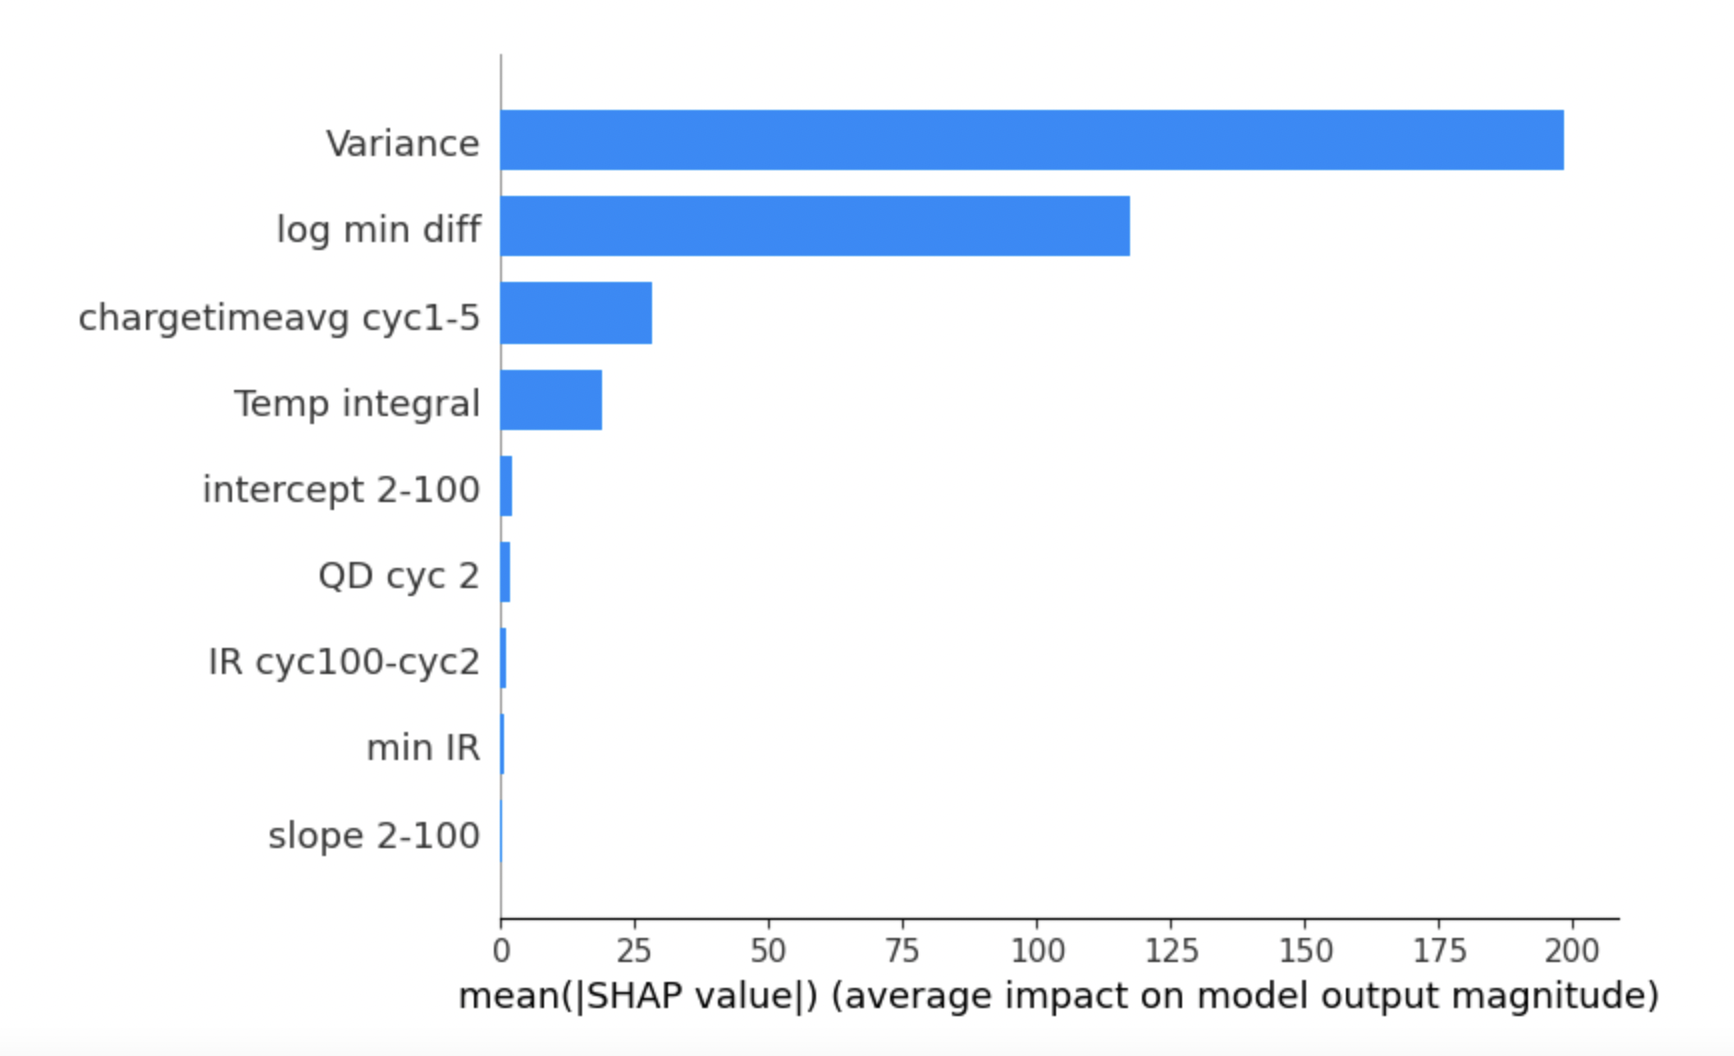
\includegraphics[width=\textwidth,height = 5cm]{figs/shap.png}
         \caption{\textbf{Top 9 feature importance scores for non time-series variables; Refer to \cite{severson2019data} for variable formulae}}
         %\label{fig:y equals x}
     \end{subfigure}
     \hfill
     \begin{subfigure}[b]{0.49\textwidth}
        \centering
        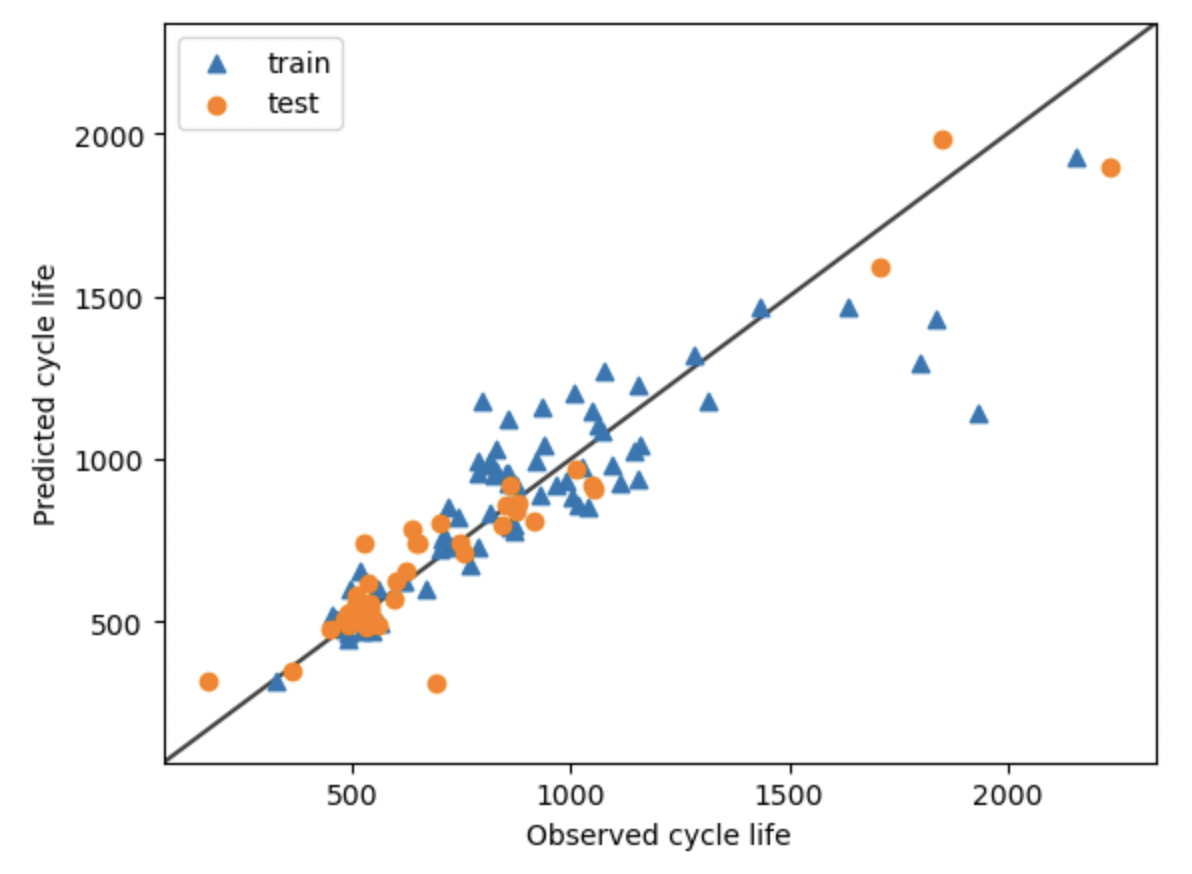
\includegraphics[width=\textwidth,height = 5cm]{figs/obspred.png}
         %\caption{\textbf{Predicted vs. Actual cycle lives}}
         %\label{fig:three sin x}
        %\caption{}
        %\label{fig:birds1}
         %\centering
         %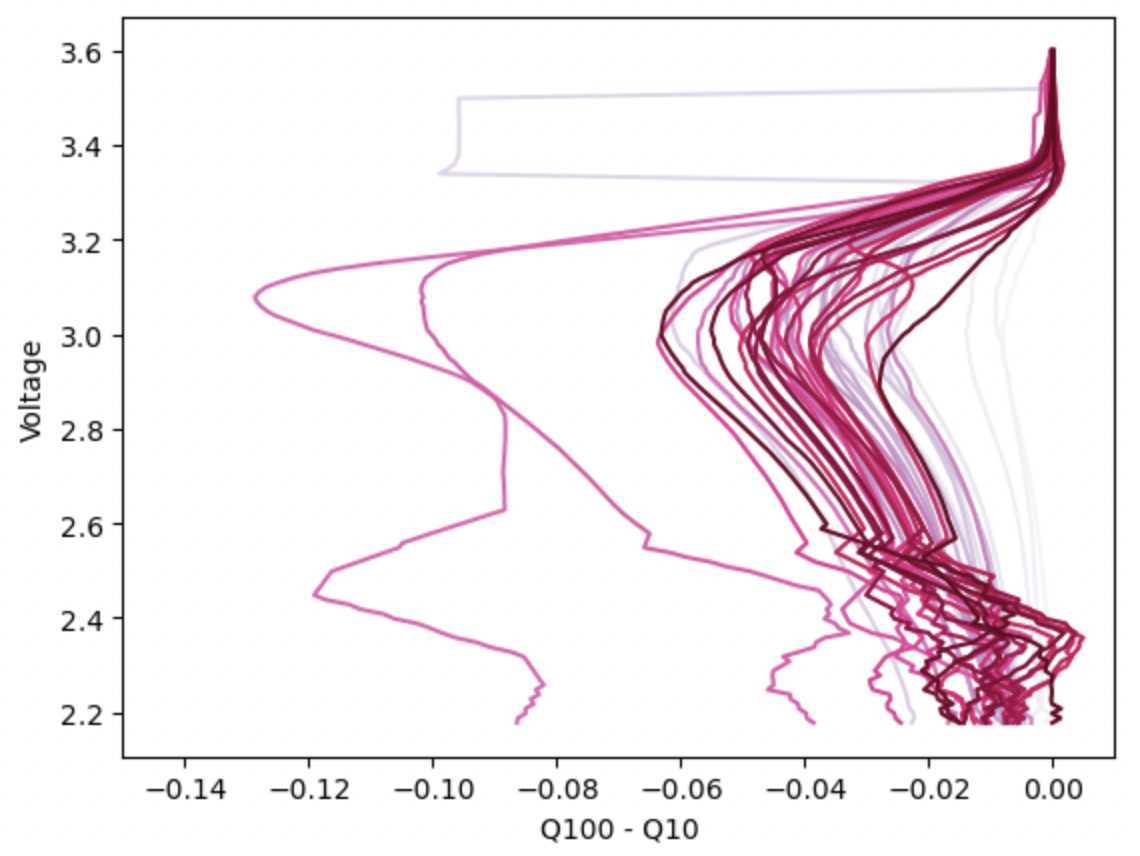
\includegraphics[width=\textwidth,height = 5cm]{figs/variance.png}
         \caption{\textbf{Predicted vs. Actual cycle lives}}
         %\label{fig:three sin x}
     \end{subfigure}
\caption{Descriptive plots for neural network approach to predicting} %cycle life}
\label{fig:birds}
\end{figure} 

\subsection{Time Series Models}
The purpose of using time series models was to predict the entire capacity degradation curve, not only the RUL as with the neural net. We experimented with both Exponential Smoothing and Auto-Regressive Integrated Moving Average (ARIMA) time series model variants. Of these two, ARIMA was the most promising variant, so this report focuses on those results. 

There were several design choices made during model development, including (a) choice of hyperparameters, (b) varying number of initialization cycles, and (c) use of exogenous variables.  

\begin{enumerate}[label=(\alph*), leftmargin=.35in]
\item \textbf{Choice of hyperparameters}: The ARIMA model consists of three parts corresponding to three defining parameters, p, d, q, where p = number of lags used, d = degree of differencing needed to make the data stationary, and q = order of moving average. We used the Box-Jenkins method with battery degradation curves from our training set to derive p (partial auto-correlation), d (differencing required to make stationary) and q (auto-correlation). We then sense checked these with results from auto-arima\cite{pmdARIMA} which performs an automatic search for the best parameters based on an information criterion (AIC). We found that p=2, d=2, q=2 worked well, and in particular that our results were very sensitive to d being at least 2. 

% the individual ACF and PACF plots of the given battery training data to determine the p and q. The d parameter was set using training set and the pmdARIMA function "ndiffs"  \cite{pmdARIMA} which estimates the number of differencing steps needed to make the data stationary. When implementing the ARIMA model we set the p and q parameters using two different methods; "auto ARIMA" which performs an automatic search for the best parameters based on an information criterion e. g AIC or BIC and, the Box-Jenkins method which is based on the properties of the ACF and PACF.

% When using auto ARIMA we restricted the range of p and q values to a range of 0-5. This was done because, through empirical testing of higher values, it was observed that the predictions did not improve, and having a greater range of values slows down auto ARIMA significantly due to the sheer increase in the number of combinations it needs to test. When using Box-Jenkins method we studied the individual ACF and PACF plots of the given battery training data to determine the p and q.  

% \item \textbf{Intialization cycles}: Original goal of 100 cycles, ... but insufficient information and so needed to expand to [xx] cycles ... we believe this limitation was due to ARIMA not being able to "pool" data across batteries. (Put earlier discussion on 300 to 100 cycles into this bullet)  From a machine learning perspective we had a separate model for each battery and therefore there was no cross-learning between batteries. This left us with a very limited amount of data to learn from, specifically only one data point per cycle. Forecasting short, non-seasonal time series is difficult. A previous study \cite{timeSeries} suggests using more advanced methods to overcome the data scarcity problem. Additionally, as the intended outcome was to predict RUL and degradation curve shape from only the first 100 cycles it became apparent that the data scarcity was severe (we were left with only 100 data points to learn from). It quickly became clear that this was impossible. Therefore, we tried predicting using more than the first 100 cycles, specifically 300 cycles.

\item \textbf{Exogenous variables}: ARIMA models can be used with or without exogenous variables. An exogenous variable is in our case a parallel time series of known values that can be imposed on the model/used as a weighted input. In the ARIMA model without exogenous variables we only considered one measurement per cycle, namely the discharge capacity $Q_D$.  

We tried adding exogenous variables to the ARIMA model, however, since the battery life cycles were of different lengths it was hard to consistently apply exogenous variables in training and testing. One approach we experimented with using exogenous data from our longest cycle life battery in the training set. However the results were mixed, particularly for shorter cycle lives. A future study could tackle this more rigorously with regressors with a normalized cycle life scale. 

\end{enumerate}

\begin{figure}[H]
\centering
    \begin{subfigure}{.5\textwidth}
  \centering
  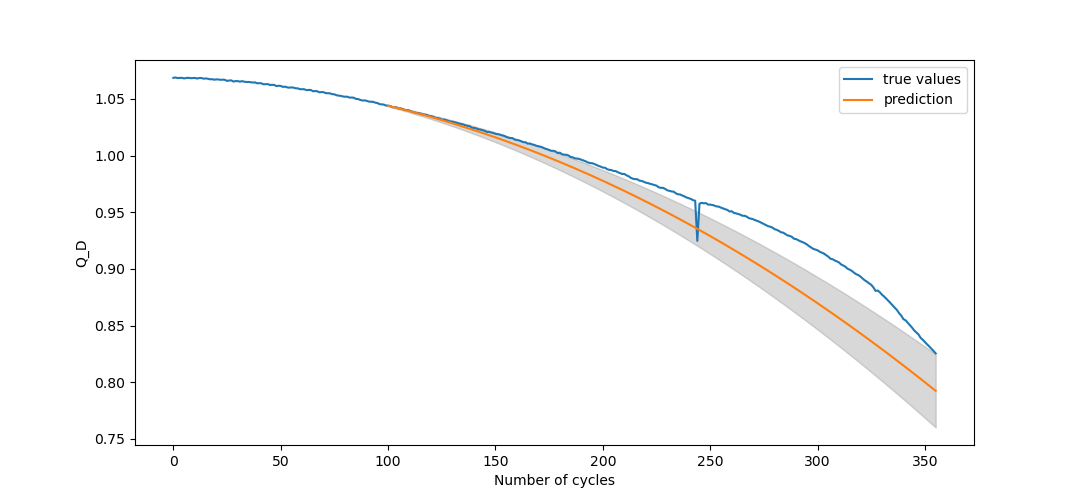
\includegraphics[height=5.2cm,width=1\linewidth]{figs/best fit 100.png}
  \caption{ARIMA, 100 cycles, on b2c3, great fit}
  \label{fig:sub1}
\end{subfigure}%
\begin{subfigure}{.5\textwidth}
  \centering
  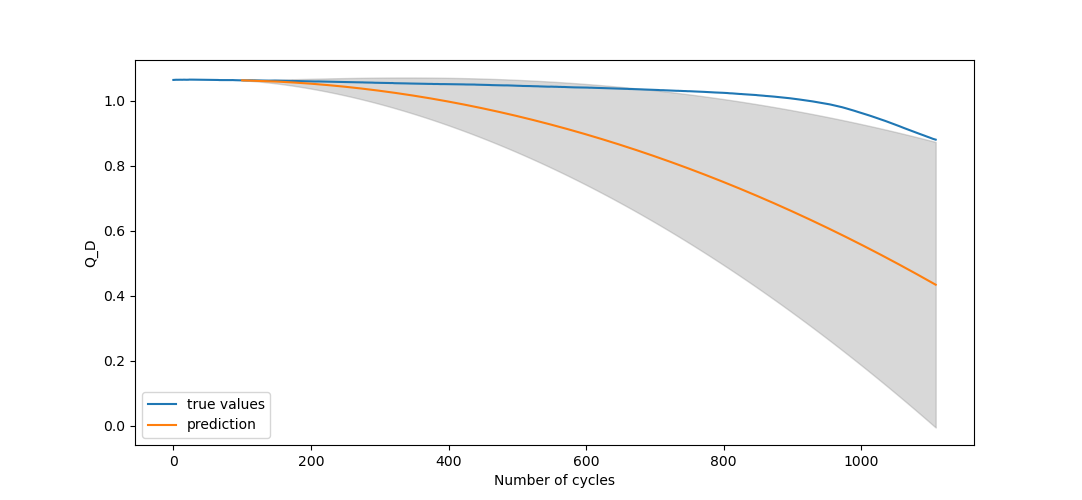
\includegraphics[height=5.2cm,width=1\linewidth]{figs/worst fit 100.png}
  \caption{ARIMA, 100 cycles, on b3c3, bad fit}
  \label{fig:sub2}
\end{subfigure}
\end{figure}

\textbf{Model evaluation}: Using ARIMA(2,2,2) and intializing each model with the first 100 cycles only, we achieve a MSE of 0.049 for SOH prediction and MAPE of 26.5\% for RUL prediction. An example of a very good and a very bad fit is presented in figures \ref{fig:sub1} and \ref{fig:sub2}. Figure \ref{fig:sub1} performs so much better than \ref{fig:sub2} because the first 100 cycles already indicate the decay trend that will follow. 


% \begin{table}[H]
%     \centering
%     \begin{tabular}{c|c}
%        mean MAPE  &  3.71\% \\
%        variance MAPE & 0.0014 \\
%        mean RMSE  &  0.050 \\
%        variance rmse & 0.0023\\
%        Cycle life prediciton error mean &  557.93
%     \end{tabular}
%     \caption{Auto ARIMA results using 300 training points and removing one outlier with cycle life < 300}
%     \label{tab:auto ARIMA 05 split}
% \end{table}

%cycle life prediction relative error mean 77.8%


\begin{comment}
From these results, we could conclude that the ARIMA model is more or less useless if used as is. However, we also tried adding exogenous variables to the ARIMA model. This created the possibility of achieving cross-learning between batteries as we could use the full degradation data from one battery as an exogenous variable when predicting on another battery. It gave a lot more data to predict on and knowledge about expected future behavior. Using the same discharge capacity data (one measurement per cycle) and one exogenous variable series it can be seen in figures (\ref{fig:sub2})-(\ref{fig:sub6}) that the predictions clearly improve when adding the exogenous variables. One can even argue that the predictions are somewhat reasonable. The exogenous variables with the greatest performance enhancement were "IR" (internal resistance) and "QD" (discharge capacity). There was no clear advantage of adding more than one exogenous variable, therefore the results using two exogenous variables are left out. It should be pointed out that the predictivity of the exogenous parameters could be questioned as it was somewhat random when they increased performance significantly, but, they never decrease performance. However, in general, the predictions using anything less than a 0.7/0.3 train/test split were seemingly random and much dependent on from which other battery the exogenous variable came. In some cases e.g see figure (\ref{fig:sub6}) great predictions where possible using as much as a 0.5/0.5 train/test split.


An attempt was made to improve the results by manually setting the ARIMA parameters using Box-Jenkins method. However, the results did, not surprisingly, not become better and the plots are therefore left out.
\end{comment}


\begin{comment}
Using the Box-Jenkins method we could not run a test on every single battery because that would be too labour intensive since the parameters are determined manually. Rather, we tried to recreate a small collection of the results that the auto ARIMA model achieved. This was done successfully which implies that the auto ARIMA model is as good as possible.
\end{comment}
\begin{comment}
**Take out below peice on exponential smoothing

The performance of the exponential smoothing model was not satisfactory. The Holt method performed better than the Holt-winter method, see figure (\ref{fig:exp_holt}) for example performance of the Holt model. Considering the much worse performance than the ARIMA models the exponential smoothing models were disregarded as predictors.


\begin{figure}[H]
\centering
    \begin{subfigure}{.5\textwidth}
  \centering
  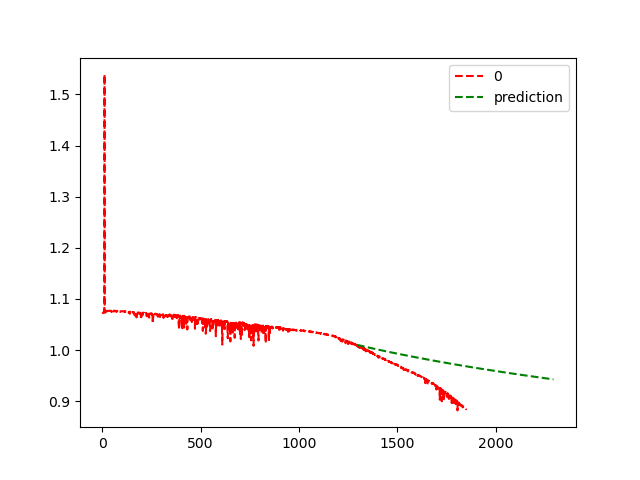
\includegraphics[width=1\linewidth]{figs/holt_exp_smooth_split07.png}
  \caption{b1c0 holt exp smoothing}
  \label{fig:exp_holt}
\end{subfigure}%
\end{figure}
\end{comment}


\subsection{Bayesian Inference Model}
We explored Bayesian Inference as a way to impose more structure (known physics) on the problem. Main idea: since we know the discharge capacity curve of each battery must be a decay curve, why don't we specify such a functional form and only ask our model to learn the shape and translation parameters. Another anticipated benefit of this approach was that we would be able to effectively pool (and learn from) data across batteries - a significant limitation of our ARIMA models.

In constructing our Bayesian Inference model we made a number of design choices, including (1) functional form, (2) parameterization and (3) selection of priors.

\begin{enumerate}[label=(\alph*), leftmargin=.35in]
    \item \textbf{Function form}: We investigated two different functional forms that described the physical behaviour we would expect in our region of interest: (a) shifted exponential decay and (b) inverse sigmoid.

    \begin{figure}[H]
        \centering
        \begin{subfigure}[b]{0.49\linewidth}
            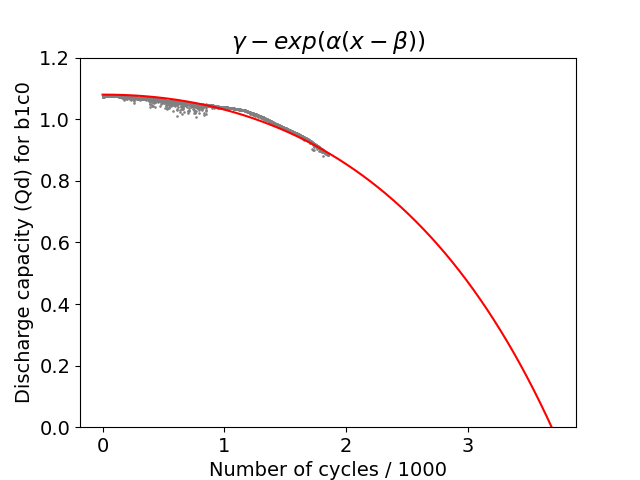
\includegraphics[height=6cm, width=\linewidth]{figs/example_exponetial_decay.png}
            \caption{Shifted exponential decay}
        \end{subfigure}
        \begin{subfigure}[b]{0.49\linewidth}
            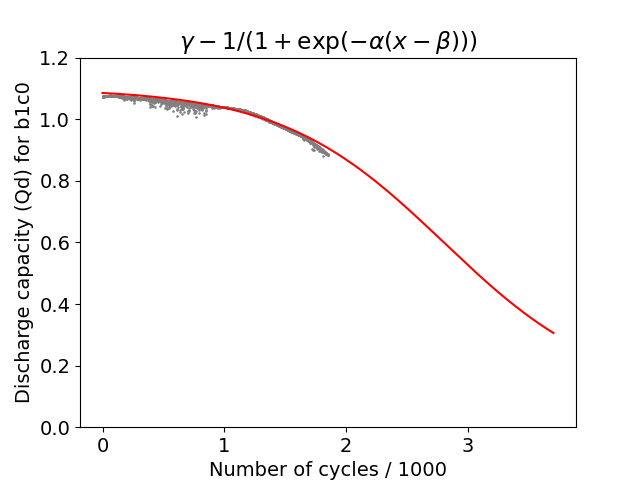
\includegraphics[height=6cm, width=\linewidth]{figs/example_inv_sigmoid.png}
            \caption{Inverse sigmoid}
        \end{subfigure}
        \caption{Comparison of functional forms fit to data for an example battery cell}
        \label{fig:funcforms}
    \end{figure}

    While the exponential decay curve seemed like a more natural fit (no inflexion point where curvature reverses), we found that the inverse sigmoid also described the data well in our region of interest (y = 0.8 to 1.2) and its parameters were more interpretable. For example, in our inverse sigmoid formulation, $\alpha$ corresponds to shape (or rate of decay), $\beta$ corresponds to horizontal translation of our sigmoid midpoint, and $\gamma$ is our y-asymptote (which we can set equal to our nominal discharge capacity for each battery). In contrast, for exponential decay, changing $\alpha$ or $\beta$ will both affect shape and horizontal translation. 
    % This leads to poor convergence of our joint posterior but also restricts our ability to interrogate what the model has learned.  
\newline
    \item \textbf{Parameterization}: Having selected a functional form, we then needed to decide how to relate our function parameters $\alpha$ (rate of decay), $\beta$ (translation) and $\gamma$ (y-asymptote) to our data features (inspired by neural network variable importance from Section 3.1). 

    \begin{itemize}
        \item \textbf{$x_1$}: nominal discharge capacity (= Qd after first cycle)
        \item \textbf{$x_2$}: variance between cycles 10 and 100 of Qd difference as a function of voltage 
        \item \textbf{$x_3$}: log of magnitude of the minimum of the Qd difference
        \item \textbf{$x_4$}: average charge time for cycles 2 through 6
        \item \textbf{$x_5$}: sum of average temperature for cycles 2 through 100
    \end{itemize}

    We choose linear models for $\alpha$ (= $a^\top x$) and $\beta$ (= $b^\top x$) based on the effectiveness of the linear model from \cite{severson2019data} for predicting RUL (closely related to translation in our case). Then for $\gamma$ we further restrict our formulation by specifying that the y-asymptote must equal the nominal discharge capacity ($x_1$).

    % \begin{align*}
    %     \alpha & = a_0 + a_1 x_1 + a_2 x_2 + a_3 x_3 + a_4 x_4 + a_5 x_5 && \text{linear model for rate of decay}\\
    %     \beta & = b_0 + b_1 x_1 + b_2 x_2 + b_3 x_3 + b_4 x_5 + b_5 x_5 && \text{linear model for horizontal translation}\\
    %     \gamma & = x_1 && \text{asymptote set to nominal discharge capacity}
    % \end{align*}

    \item \textbf{Prior specification}: We make an assumption that our labels $y$ (discharge capacity for each cycle for each battery) are generated from a normal distribution with mean $\hat{y}$ (our predictions based on learned parameters) and variance $\sigma^2$ (which we learn as a parameter).
    $$ y \sim \text{Normal}\left(\gamma - \frac{1}{1+\exp(-\alpha(x-\beta))}, \quad \sigma^2\right)$$

    For our model parameters, we impose informative priors on $a_0, b_0$ based on aggregate analysis of our data: $a_0 \sim N(3,1)$ and $b_0 \sim N(2,1)$, and weakly informative (standard normal) priors on the remaining $a_i, b_i$ parameters since we did not have pre-existing intuition for these relationships. Finally, for variance, we impose a more traditional gamma prior $\sigma^2 \sim \text{Gamma}(1, 2)$.

\end{enumerate}

To sample from our joint posterior, we use the Hamiltonian Monte Carlo No U-Turn sampling method (Stan in-built). See Appendix 5.2 for detailed analysis of posterior marginals and sampling efficiency. \newline

\textbf{Model evaluation}: On out-of-sample test data, our model achieves MSE of 0.015 for SOH prediction and MAPE of 33.5\% for RUL prediction. While the curve fit is an improvement on our time series models, the RUL is worse.

    \begin{figure}[H]
        \centering
        \begin{subfigure}[b]{0.49\linewidth}
            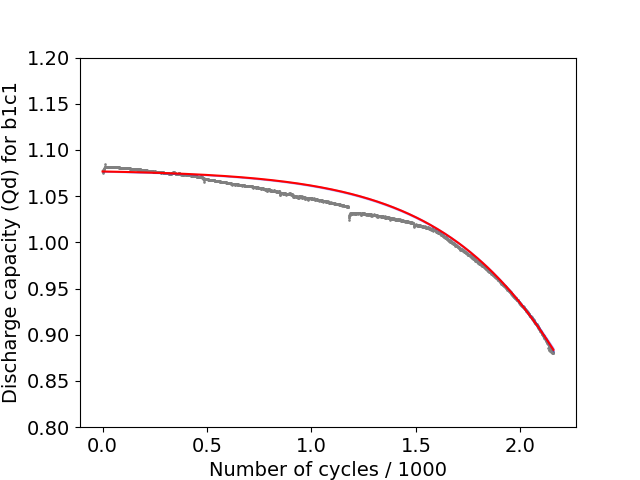
\includegraphics[height=6cm,width=\linewidth]{figs/bayes_plot_with_error_b1c1.png}
            \caption{SOH MSE = 0.0008, RUL MAPE = 1.5\%}
            \label{fig:bayessub1}
        \end{subfigure}
        \begin{subfigure}[b]{0.49\linewidth}
            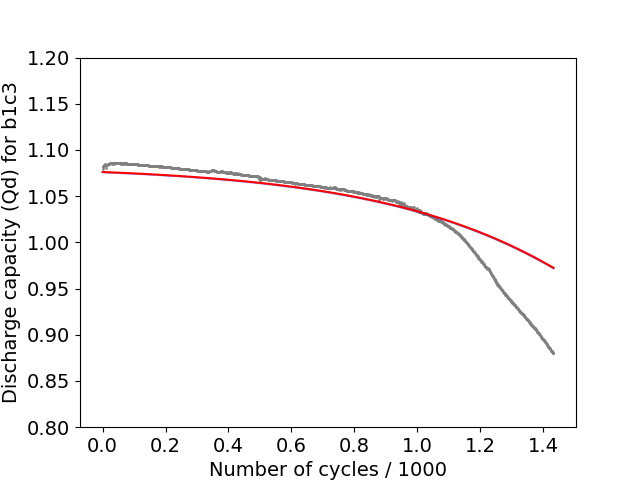
\includegraphics[height=6cm,width=\linewidth]{figs/bayes_plot_with_error_train_b1c3.png}
            \caption{SOH MSE = 0.022, RUL MAPE = 38.5\%}
            \label{fig:bayessub2}
        \end{subfigure}
        \caption{Predicted discharge capacity over normalized cycle life}
        \label{fig:bayespred}
    \end{figure}
Our model predicts well for batteries with mid-long cycle lives (Figure \ref{fig:bayessub1}), but often overshoots for short cycle life batteries (e.g. Figure \ref{fig:bayessub2}). This is partly due us having so few short cycle life training observations (variance), but also may be indicative of inflexibility in the model parameterization (bias). For example, our linear model for the shape and translation terms might be too simplistic. Examples like Figure \ref{fig:bayessub2} disproportionately impact the RUL MAPE performance relative to our ARIMA model. 

\section{Conclusions}
In general, while we were able to confirm that a relatively simple model can predict RUL accurately (MAPE $\approx$ 11\%), finding a white box model to predict both RUL and the SOH curve proved much more difficult. This is likely due to the error propagation in predicting the decay curve, which causes predicted RUL (the predicted decay curve endpoint in this case) to either over or undershoot drastically. Our Bayesian and ARIMA models were each best on different metrics: Bayesian for SOH MSE (0.015 vs 0.049) and ARIMA for RUL MAPE (26.5\% vs 33.5\%).  

There are a few areas of future study that would be interesting to pursue as next steps. First, given the partial success of the ARIMA models, we could try using a Long Short Term Memory (LSTM) Neural Network to see if we can improve predictions for the decay curve. This would no longer be a white box model that could be used in online systems, but might still be useful for offline use cases. Second, our ARIMA models struggled when the first 100 cycles were flat, which suggests we could improve by adding well-chosen exogneous variables that encode an downwards trend (or inflexion point). Given the varying number of cycles for each battery prediction, any exogneous variable would need to be flexible in length and therefore model generated (e.g. regressors). Third, one idea for improving our bayesian formulation would be to refine the parameterization for shape and translation of our inverse sigmoid. We currently use a linear model, but a deeper understanding of the physics involved might lead us to specify something more complex (e.g. with interaction terms).

% The high variance in performance of the auto ARIMA model is due to the fact that, for all batteries, we could only predict using a maximum number of datapoints as that of the total amount of datapoints in the cycle life of the shortest battery life (which was about 150). This lead to very poor predictions on the batteries with longer cycle lifes. If one would use the estimated cycle life derived using either the neural network or the GDA model and then decide to predict the discharge curve shape after a certain percentage of the predicted cycle life, one could expect better results.

\newpage
\section{Appendix}
\subsection{Data exploration}

\textbf{Discharge capacity vs cycle number}. Our goal is to predict the discharge curves below given information from the first 50-100 cycles. A few things to note. First, the batteries in our population are either rated at 1.1 Ah or 1.05 Ah nominal capacity. By nominal here we mean manufacturer rated initial capacity. Second, in practice, our initial discharge capacity rarely perfectly matches the nominal capacity rating and so instead of two discrete starting points at 1.1 and 1.05, our starting points range continuously in that range. Third, our data is meant to reflect cycling each battery from its initial capacity to 80\% of its nominal. This explains the two distinct end points we observe in the right hand chart at 0.88 Ah and 0.84 Ah, the 80\% thresholds of 1.1 Ah and 1.05 Ah nominal capacities respectively. Last, in plotting these curves we identified some obvious outliers. Batteries in the left hand plot with capacities either above 1.2 or below 0.8 are erroneous measurements that we remove from the data before training.  

    \begin{figure}[H]
        \centering
        \begin{subfigure}[b]{0.49\linewidth}
            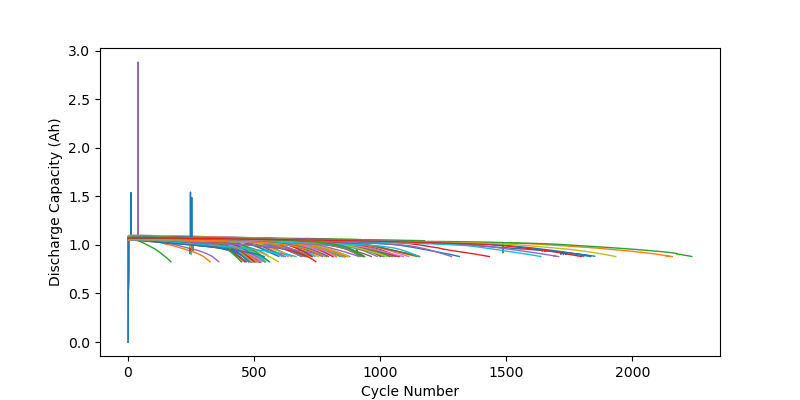
\includegraphics[width=\linewidth]{figs/discharge_capacity_by_cycle.png}
            \caption{Complete dataset}
        \end{subfigure}
        \begin{subfigure}[b]{0.49\linewidth}
            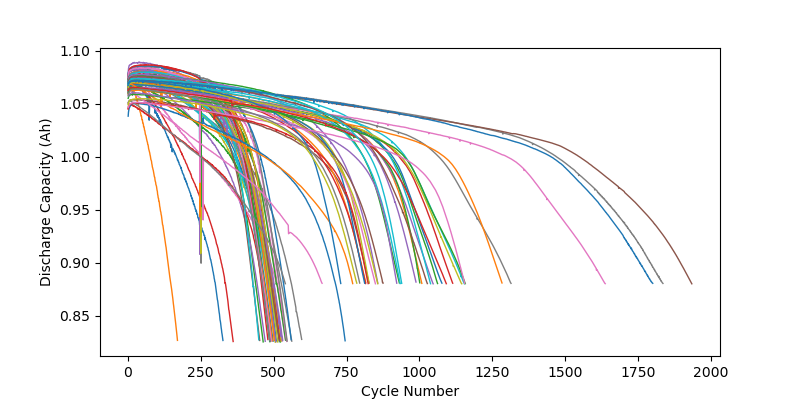
\includegraphics[width=\linewidth]{figs/discharge_capacity_by_cycle_remove_outliers.png}
            \caption{Outliers removed}
        \end{subfigure}
        \caption{Discharge capacity by cycle number for 124 batteries}
        \label{fig:3a}
    \end{figure}

\textbf{Distribution of our target variable}. Cycle life is the number of cycle it takes for a given battery to reach 80\% of its nominal capacity. This is our target variable. When plotting the complete dataset we identified a skewed normal distribution. Ideally we want to roughly maintain this distribution for our validation and test data. To achieve this we re-used logic from "Data-driven prediction of battery cycle life before capacity degradation" \cite{severson2019data} to split our train, validation and test data.

    \begin{figure}[H]
        \centering
        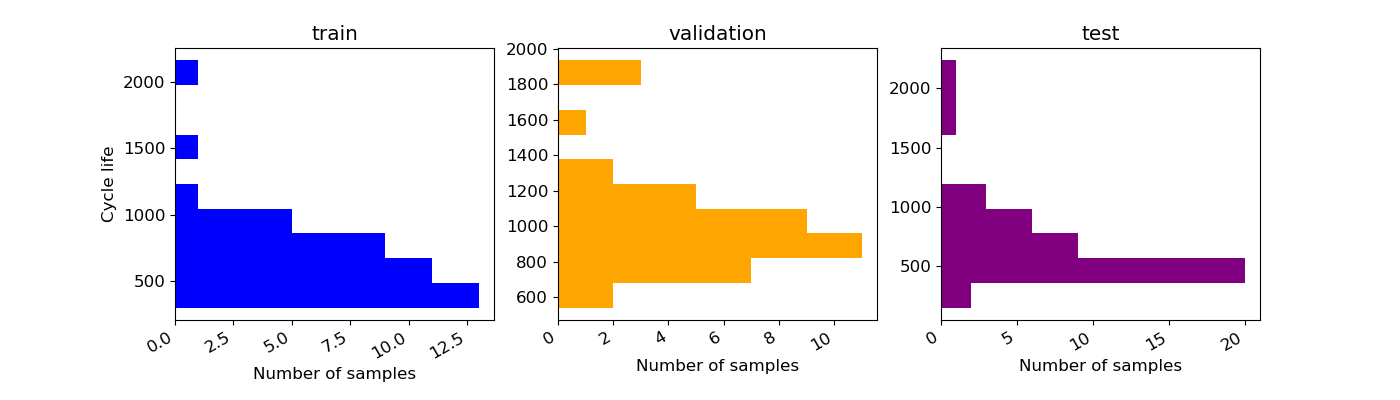
\includegraphics[scale=0.5] {figs/histogram_cycle_life_traintest.png}
        \caption{Distribution of target for train, validation and test data}
        \label{fig:1b}
    \end{figure}

\textbf{Applied current and charge cycle}. The charts below illustrate current, charge capacity, and  discharge capacity for all cycles of an example battery data point (ref: b1c0). We can immediately confirm that the vast majority of cycles follow similar charge profiles. In particular, applying positive current (charging) for first 500-700 time steps, then switching to an applied negative current (discharging) until depleted at the end of the cycle. The charge capacity (Qc) and discharge capacity (Qd) charge plots also show this transition, with Qc increasing up until the changeover to negative applied current, and Qd increasing only after the changeover.

    \begin{figure}[H]
        \centering
        \begin{subfigure}[b]{0.32\linewidth}
            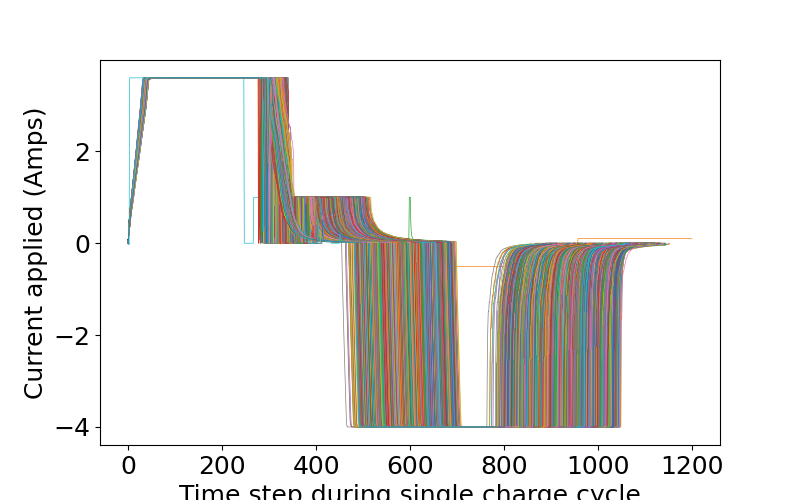
\includegraphics[width=\linewidth]{figs/b1c0_iapp_intracycle.png}
            \caption{Applied current}
        \end{subfigure}
        \begin{subfigure}[b]{0.32\linewidth}
            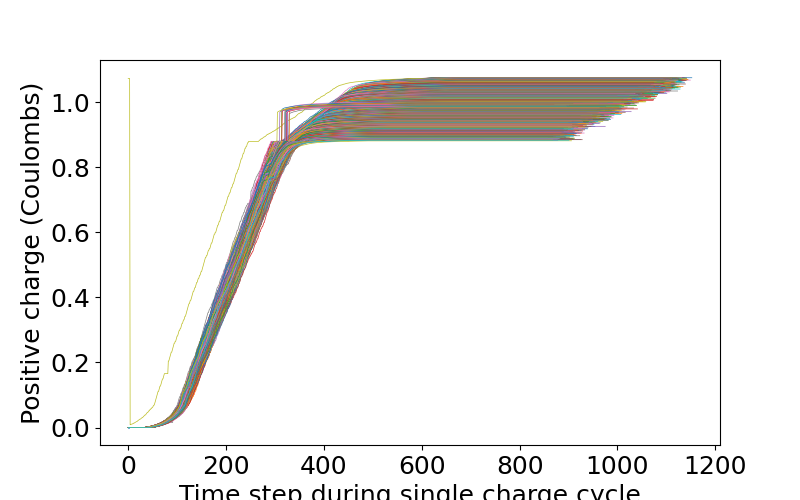
\includegraphics[width=\linewidth]{figs/b1c0_qc_intracycle.png}
            \caption{Charge capacity (Qc)}
        \end{subfigure}
        \begin{subfigure}[b]{0.32\linewidth}
            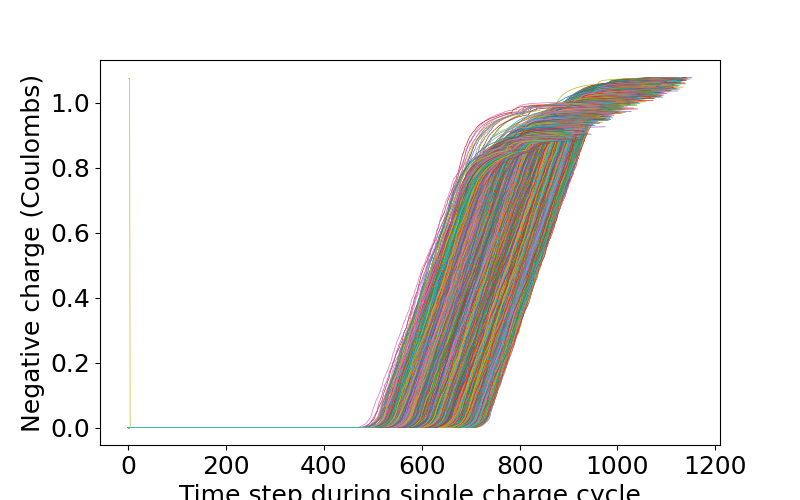
\includegraphics[width=\linewidth]{figs/b1c0_qd_intracycle.png}
            \caption{Discharge capacity (Qd)}
        \end{subfigure}
        \caption{Charge and discharge cycles for an example battery (ref: b1c0)}
        \label{fig:1c}
    \end{figure}

We also investigated how voltage and temperature vary over the cycles of the same example battery. It is interesting to note that while temperature has a roughly gaussian distribution throughout any given cycle, the voltage measure has almost no variance during charge but significant variance across cycles during discharge. 

    \begin{figure}[H]
        \centering
        \begin{subfigure}[b]{0.49\linewidth}
            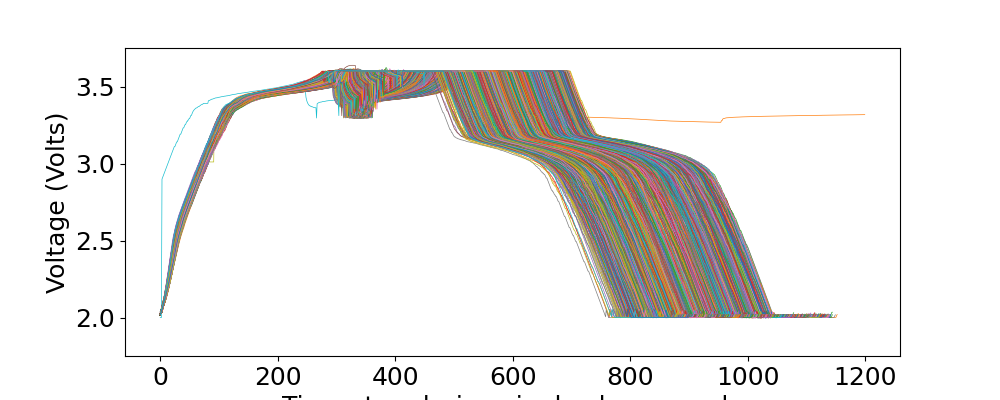
\includegraphics[width=\linewidth]{figs/b1c0_voltage_intracycle.png}
            \caption{Voltage (volts)}
        \end{subfigure}
        \begin{subfigure}[b]{0.49\linewidth}
            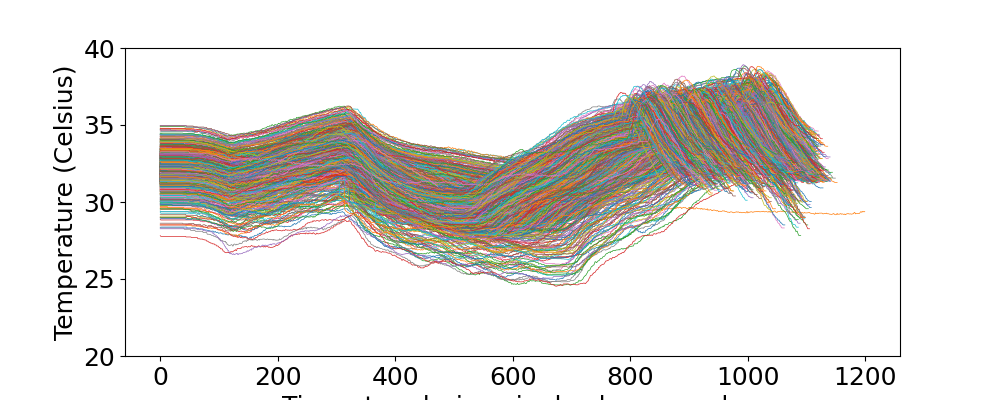
\includegraphics[width=\linewidth]{figs/b1c0_temp_intracycle.png}
            \caption{Temperature (degrees celsius)}
        \end{subfigure}
        \caption{Voltage and temperature over cycles for an example batter (ref: b1c0)}
        \label{fig:1d}
    \end{figure}
    
\textbf{Correlation with cycles @ 5\% fade}. Finally, we wanted to directly plot some measure of capacity fade (in this case number of cycles to reach 5\% decrease from nominal) during the initial cycles against cycle life to see if we can recover the correlated behaviour we expect between early trajectory and end point of the discharge capacity curve. Encouragingly, we see the two are highly correlated, achieving a pearson correlation coefficient of approximately 0.94.

    \begin{figure}[H]
        \centering
        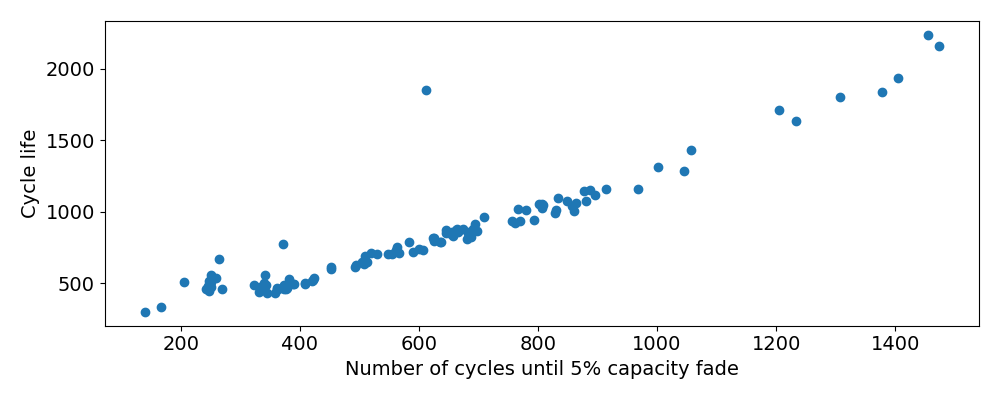
\includegraphics[scale=0.5] {figs/correlation_cycle_life_vs_5pct_fade.png}
        \caption{Scatter plot demonstrating correlation between cycle life and 5\% capacity fade}
        \label{fig:1e}
    \end{figure}

\newpage
\subsection{Hamiltonian Monte Carlo Sampling}

\textbf{Sampled posterior marginals}. Our sampled posterior marginal histograms are what we use to make predictions. We can take the mean from each (converges to MLE for large training dataset) or use information from these distributions to generate predictions that reflect prediction uncertainty (eg. +/- standard deviation). 

    \begin{figure}[H]
        \centering
        \begin{subfigure}[b]{0.49\linewidth}
            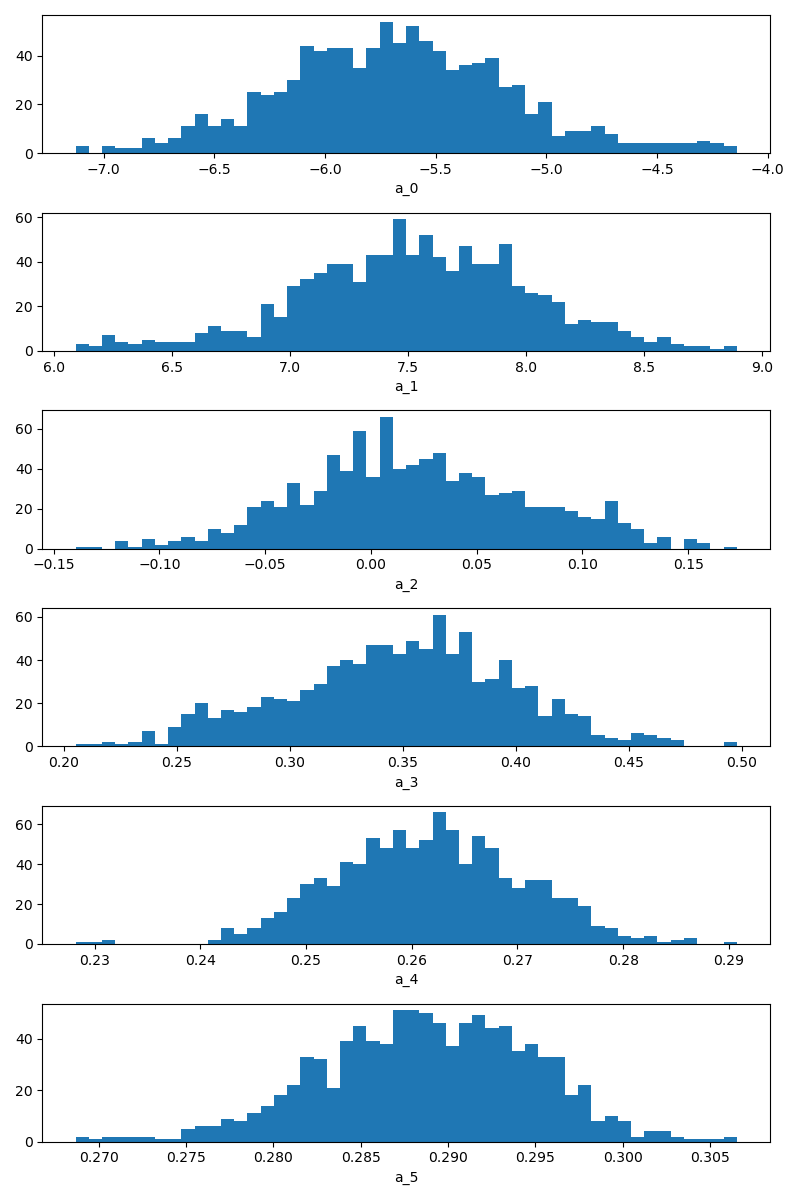
\includegraphics[width=\linewidth]{figs/bayes_alpha_sampled_histogram.png}
            \caption{Rate of decay parameters ($\alpha$)}
        \end{subfigure}
        \begin{subfigure}[b]{0.49\linewidth}
            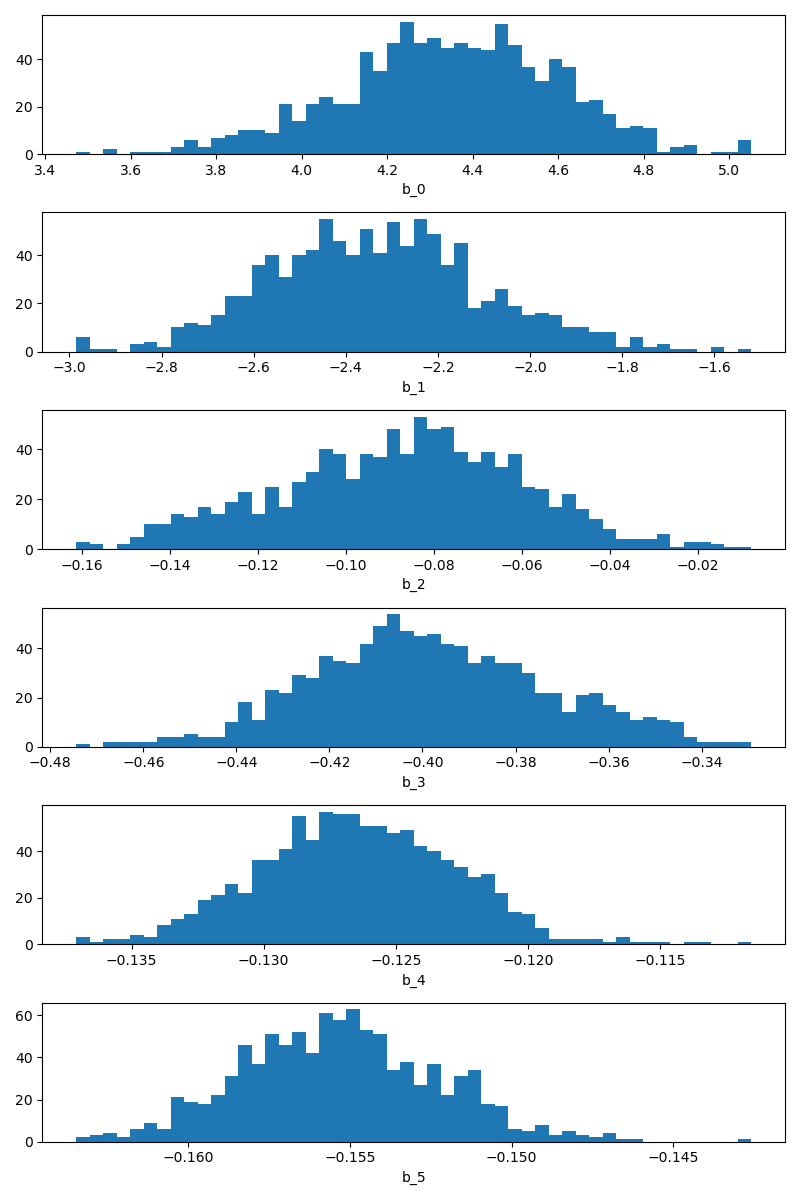
\includegraphics[width=\linewidth]{figs/bayes_beta_sampled_histogram.png}
            \caption{Translation parameters ($\beta$)}
        \end{subfigure}
        \caption{Sampled posterior marginals for alpha and beta linear model parameters}
        \label{fig:bayeshist}
    \end{figure}

\newpage
\textbf{Sampling efficiency}. Our trace plots (only samples after burn-in shown) give a sense of the path that our MCMC sampler (No U-turn Hamilton Monte Carlo) took through the posterior space. AS we had hoped, these show reasonable variation, but no major divergences or long periods of repeated value where the sampler was stuck.

    \begin{figure}[H]
        \centering
        \begin{subfigure}[b]{0.49\linewidth}
            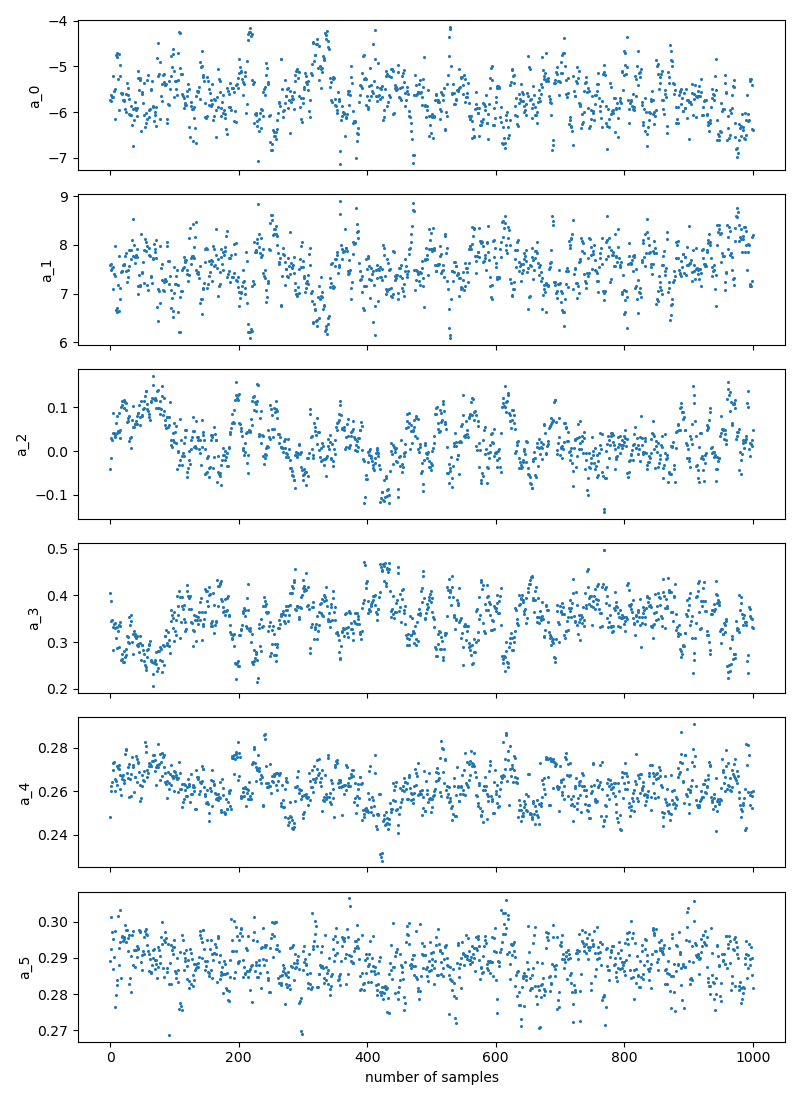
\includegraphics[width=\linewidth]{figs/bayes_alpha_sampled_traceplot.png}
            \caption{Rate of decay parameters ($\alpha$)}
        \end{subfigure}
        \begin{subfigure}[b]{0.49\linewidth}
            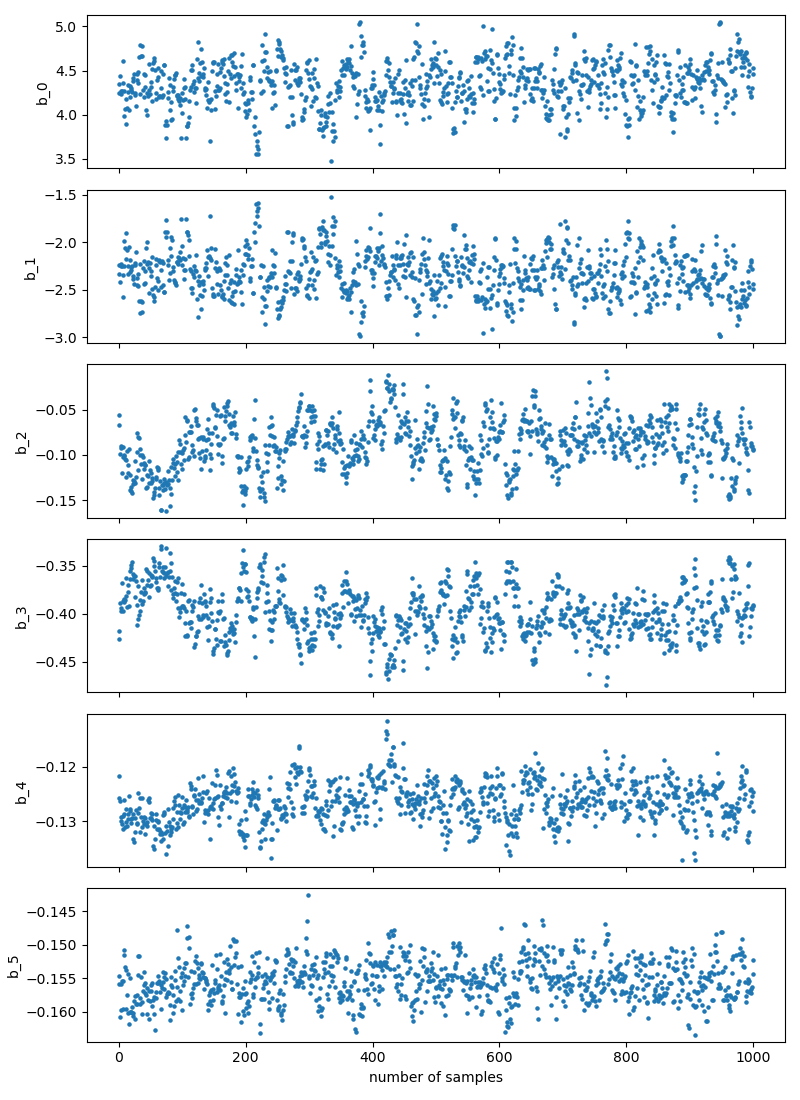
\includegraphics[width=\linewidth]{figs/bayes_beta_sampled_traceplot.png}
            \caption{Translation parameters ($\beta$)}
        \end{subfigure}
        \caption{Trace plot of HMC sampling for alpha and beta linear model parameters}
        \label{fig:bayestrace}
    \end{figure}

When considering sampling efficiency we also consider auto-correlation between samples. Ideally, we want to take gradient steps through the posterior space such that we maximize the number of "effective" (uncorrelated) samples. In this case, from 1,000 draws we generate ~175 effective samples.

% \subsection{GDA, an alternative model}
% We built a GDA model for RUL/cycle life predictions as a comparison to the neural net and because it had not, to our knowledge, been done before. Furthermore, it could also be reasonable to believe that the different batteries come from some normal distributions with respect to cycle life. We created one class per 100th increase in cycle life, i. e 19 separate classes, equally spaced between 100 and 1900, and tried to assign each battery in the test set to one of these classes. The model took 27 different features per cycle for each battery and tried to classify the cycle life based on the first 100 cycles. The features were not scaled. As labels, we used the known cycle life of each battery. Specifically we used an LDA (linear discriminant analysis) model implemented using the SKlearn LinearDiscriminantAnalysis class \cite{scikit-learn}. The results are presented in \ref{fig:GDA_scatter}. We notice an accuracy similar to the neural network with a MAPE of $13.14\%$. However, it should be emphasized that we did predictions on discrete classes and not on the exact cycle life.

% \begin{figure}[H]
%     \centering
%     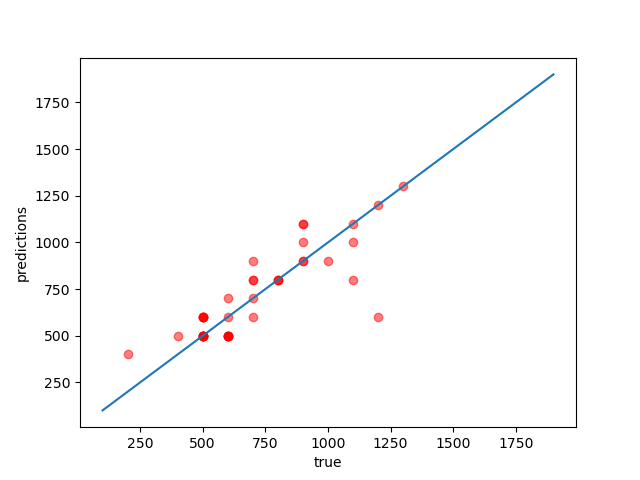
\includegraphics[scale=0.6]{figs/GDA scatter plot.png}
%     \caption{GDA results scatter plot}
%     \label{fig:GDA_scatter}
% \end{figure}

\newpage
\large {\textbf{Contributions}}

Julian owned development of the Bayesian Inference model. Hampus owned development of the ARIMA and Exponential Smoothing models. Karthik owned development of the Neural Network model. Everyone contributed to data exploration, fit evaluation methodology and brainstorming on / sense checking each others' results and design choices.

\bibliography{citation}
\end{document}
